\chapter{$L$-bounded cuts}

In this chapter we will consider a new problem which is length bounded cuts. This problem is NP-hard.

\begin{itemize}[]
	\item \textbf{INPUT} $G = (V,E)$, $s,t \in V$, $L \in \N$.
	\item \textbf{OUTPUT} $F \subseteq E$ such that $d_{G \setminus F}(s,t) > L$.
	\item \textbf{OBJECTIVE} $\min (|F|)$.
\end{itemize}

Lets see an easy example of a graph $G$ as shown on the picture \ref{l-bounded cut} and for $L = 4$. There can actually be two minimal $L$-bounded cuts. The \textcolor{orange}{first} one is actually not a "real" cut, but the \textcolor{cyan}{second} one is.

\begin{figure}[!ht]\centering
	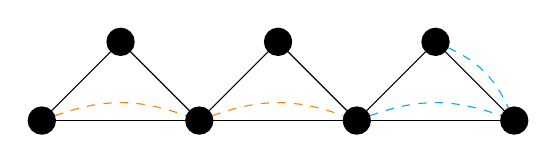
\begin{tikzpicture}[node distance={10mm}, main/.style = {draw, thick, fill, circle}]
		\node[main] (1) {};
		\node[right of = 1] (1a) {};
		\node[main, above of = 1a] (1b) {};
		\node[main, right of = 1a] (2) {};
		\node[right of = 2] (2a) {};
		\node[main, above of = 2a] (2b) {};
		\node[main, right of = 2a] (3) {};
		\node[right of = 3] (3a) {};
		\node[main, above of = 3a] (3b) {};
		\node[main, right of = 3a] (4) {};
		
		\draw (1) edge (2);
		\draw (1) edge (1b);
		\draw (1b) edge (2);
		
		\draw (2) edge (3);
		\draw (2) edge (2b);
		\draw (2b) edge (3);
		
		\draw (3) edge (4);
		\draw (3) edge (3b);
		\draw (3b) edge (4);
		
		\draw[color = orange, bend left = 20, dashed] (1) edge (2);
		\draw[color = orange, bend left = 20, dashed] (2) edge (3);
		
		\draw[color = cyan, bend left = 20, dashed] (3) edge (4);
		\draw[color = cyan, bend left = 20, dashed] (3b) edge (4);
	\end{tikzpicture}
	\caption{Example of $L$-bounded cut. The cut is drawn by a multiple dashed edge.}
	\label{l-bounded cut}
\end{figure}


\section{$L$-bounded flow}

For $L$-bounded cut there is also the opposite problem which is in P and it is the $L$-bounded flow.

\begin{itemize}[]
	\item \textbf{INPUT} $G = (V,E)$, $s,t \in V$, $L \in \N$.
	\item \textbf{OUTPUT} Flow between $s-t$ that can be decomposed into paths of length $\leq L$.
	\item \textbf{OBJECTIVE} $\max$ the flow.
\end{itemize}

We will also show us an example for a graph $G$ depicted on the picture \ref{l-bounded flow} for $L = 3k$. We may see that $L$-cut is $k+1$ since we may delete \textcolor{cyan}{these edges} but also \textcolor{orange}{the bottom ones}. On the other hand $L$-flow is at most 2.

\begin{figure}[!ht]\centering
	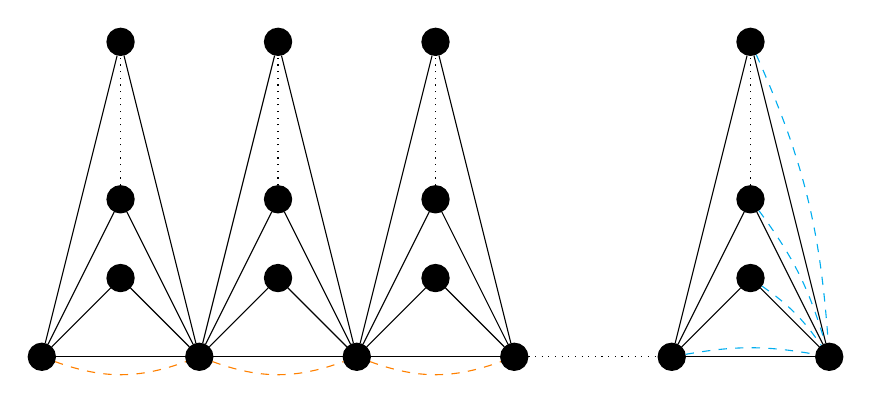
\begin{tikzpicture}[node distance={10mm}, main/.style = {draw, thick, fill, circle}]
		\node[main] (1) {};
		\node[right of = 1] (1a) {};
		\node[main, above of = 1a] (1b) {};
		
		\node[main, above of = 1b] (1c) {};
		\node[above of = 1c] (1d) {};
		\node[main, above of = 1d] (1e) {};
		
		\node[main, right of = 1a] (2) {};
		\node[right of = 2] (2a) {};
		\node[main, above of = 2a] (2b) {};
		
		\node[main, above of = 2b] (2c) {};
		\node[above of = 2c] (2d) {};
		\node[main, above of = 2d] (2e) {};
		
		\node[main, right of = 2a] (3) {};
		\node[right of = 3] (3a) {};
		\node[main, above of = 3a] (3b) {};
		
		\node[main, above of = 3b] (3c) {};
		\node[above of = 3c] (3d) {};
		\node[main, above of = 3d] (3e) {};
		
		\node[main, right of = 3a] (4) {};
		
		\node[right of = 4] (phantom) {};
		
		\node[main, right of = phantom] (k) {};
		\node[right of = k] (ka) {};
		\node[main, above of = ka] (kb) {};
		
		\node[main, above of = kb] (kc) {};
		\node[above of = kc] (kd) {};
		\node[main, above of = kd] (ke) {};
		
		\node[main, right of = ka] (k+1) {};
		
		\draw (1) edge (2);
		\draw (1) edge (1b);
		\draw (1b) edge (2);
		\draw (1) edge (1c);
		\draw (1c) edge (2);
		\draw (1) edge (1e);
		\draw (1e) edge (2);
		\draw[dotted] (1c) edge (1e);
		
		\draw (2) edge (3);
		\draw (2) edge (2b);
		\draw (2b) edge (3);
		\draw (2) edge (2c);
		\draw (2c) edge (3);
		\draw (2) edge (2e);
		\draw (2e) edge (3);
		\draw[dotted] (2c) edge (2e);
		
		\draw (3) edge (4);
		\draw (3) edge (3b);
		\draw (3b) edge (4);
		\draw (3) edge (3c);
		\draw (3c) edge (4);
		\draw (3) edge (3e);
		\draw (3e) edge (4);
		\draw[dotted] (3c) edge (3e);
		
		\draw[dotted] (4) edge (k);
		
		\draw (k) edge (k+1);
		\draw (k) edge (kb);
		\draw (kb) edge (k+1);
		\draw (k) edge (kc);
		\draw (kc) edge (k+1);
		\draw (k) edge (ke);
		\draw (ke) edge (k+1);
		\draw[dotted] (kc) edge (ke);
		
		\draw[dashed, color = cyan, bend left = 10] (k) edge (k+1);
		\draw[dashed, color = cyan, bend left = 10] (kb) edge (k+1);
		\draw[dashed, color = cyan, bend left = 10] (kc) edge (k+1);
		\draw[dashed, color = cyan, bend left = 10] (ke) edge (k+1);
		
		\draw[dashed, color = orange, bend right = 20] (1) edge (2);
		\draw[dashed, color = orange, bend right = 20] (2) edge (3);
		\draw[dashed, color = orange, bend right = 20] (3) edge (4);
	\end{tikzpicture}
	\caption{Example of $L$-bounded flow. Where there is $2k$ bottom vertices and $k$ upwards in each triangle. Cuts are represented by multi edges that are dashed.}
	\label{l-bounded flow}
\end{figure}

\begin{observ}
	Every $L$-bounded $s-t$ path uses at least $k$-edges from the bottom so max $L$-flow is at most 2.
\end{observ}

Therefore the difference between $L$-cut and $L$-flow can be at least $\sqrt{n}$.

\section{Approximation for $L$-cut}

Consider the following LP relaxation. Alternatively the ILP will surely solve the problem. Lets denote $\mathcal{P}_L$ as the set of all $L$-bounded $s-t$ paths.

$$
\begin{aligned}
	\min \sum_{e \in E} x_e & \\
	\sum_{x \in p} x_e \geq 1 & \quad \forall p \in \mathcal{P}_L \\
	x_e \geq 0 & \quad \forall e \in E
\end{aligned}
$$

We may ask ourselves what is the integrality gap? We can create one simple algorithm for solving such problem.

\begin{algorithm}
	\caption{$L$-bounded approximation}
	\begin{algorithmic}[1]
		\Require $G = (V,E)$
		\Ensure $L$-bounded cut.
		\While{$\exists L$-bounded $s-t$ path in $G$}
			\State Remove all edges of $p$.
		\EndWhile
	\end{algorithmic}
\end{algorithm}

\begin{observ}
	While the OPT $\geq k$ therefore it is $L$-approximation. Since the $k$ is the number of $L$-paths.
\end{observ}

Also we can see what is the is the dual to this LP. Which will indeed solve $L$-flows.
% TODO This may be changed.
$$
\begin{aligned}
	\max \sum_{p \in \mathcal{P}_L} f_p &\\
	\sum_{p \in \mathcal{P}_L, e \in p} f_p & \forall e \in E\\
	f_p \geq 0 & \forall p \in \mathcal{P}_L
\end{aligned}
$$